\documentclass[letterpaper]{article}
% \IEEEoverridecommandlockouts
% The preceding line is only needed to identify funding in the first footnote. If that is unneeded, please comment it out.
\usepackage{cite}
\usepackage[portuges,brazil,english]{babel}
\usepackage{amsmath,amssymb,amsfonts}
\usepackage{graphicx}
\usepackage{textcomp}
\usepackage[utf8]{inputenc}
\usepackage[T1]{fontenc}
\usepackage{amsmath}
\usepackage{nccmath}
\usepackage{hyperref}
\usepackage{multirow}
\def\BibTeX{{\rm B\kern-.05em{\sc i\kern-.025em b}\kern-.08em
    T\kern-.1667em\lower.7ex\hbox{E}\kern-.125emX}}
\usepackage{xcolor}
\usepackage{listings}
\usepackage{float}

\renewcommand{\lstlistingname}{Trecho}
\renewcommand{\lstlistlistingname}{Lista de \lstlistingname s}

\definecolor{codegreen}{rgb}{0,0.6,0}
\definecolor{codegray}{rgb}{0.85,0.85,0.85}
\definecolor{codepurple}{rgb}{0.58,0,0.82}
\definecolor{codeblack}{rgb}{0,0,0}

\lstdefinestyle{codigo}{
    backgroundcolor=\color{codegray},   
    commentstyle=\color{codegreen},
    keywordstyle=\color{magenta},
    numberstyle=\tiny\color{codeblack},
    stringstyle=\color{codepurple},
    basicstyle=\ttfamily\footnotesize,
    breakatwhitespace=false,         
    breaklines=true,                 
    captionpos=b,                    
    keepspaces=true,                 
    numbers=left,                    
    numbersep=5pt,                  
    showspaces=false,                
    showstringspaces=false,
    showtabs=false,                  
    tabsize=4
}

\lstset{style=codigo}    
    
\begin{document}

\title{FairPEK - Documentação}
\author{Instalação}

\maketitle

\section{Introdução}

Esta documentação foi criada com o objetivo de guiar o Desenvolvedor de Software a entender, configurar e manter este sistema, que é dividido em 4 módulos principais:

\begin{itemize}
    \item {\textbf{Engenharia de dados:}} Módulo criado com o objetivo de simular processos de transformação e limpeza de dados.
    \item {\textbf{Módulo de Machine Learning:}} Módulo que executa um Pipeline capaz de automatizar uma aplicação de Machine Learning (ML), com estágios de preparação de dados (Pré-processamento), treinamento (Processamento) e avaliação dos resultados (Pós-processamento) para a geração de um modelo final.
    \item {\textbf{Gerenciador Autonômico:}} Módulo contendo um loop, baseado na arquitetura MAPE-K, que controla o Módulo de ML como um Elemento Gerenciado para automatizar parte das atividades a serem executadas.
    \item {\textbf{Interface:}} : Módulo cujo objetivo é prover uma experiência de usuário mais simples e intuitiva para configurar e iniciar o Gerenciador Autonômico. É composto por dois componentes:
    \begin{itemize}
        \item {\textbf{Frontend:}} Componente visual, exibido em um navegador.
        \item \textbf{{Backend:}} Componente no qual o Frontend estabelece comunicação para obter os dados e montar o visual corretamente, de forma que corresponda a configurações utilizadas pelo Gerenciador Autonômico.
    \end{itemize}
\end{itemize}

\section{Programas necessários para instalação}

\begin{itemize}
    \item {\textbf{Python:}} É a linguagem de programação utilizada para montar e executar todos os módulos com a exceção do Frontend da interface. É disponível no site \url{https://www.python.org/} e é necessária a versão \textbf{3.8}, \textbf{3.9} ou \textbf{3.10}. Versões inferiores ou iguais a \textbf{3.7} a superiores ou iguais a \textbf{3.11} apresentaram problemas de compatibilidade devido a mudanças de design.
    \item {\textbf{Node.js:}} É o programa necessário para montar o Frontend da interface. É disponível no site \url{https://nodejs.org/} e foi testado na versão \textbf{16.14.2}, embora outras versões podem ser executadas sem problemas de compatibilidade.
    \item {\textbf{Git:}} É o programa necessário para realizar o download do código-fonte e realizar atualizações no mesmo. É disponível no site \url{https://git-scm.com/} e foi testado na versão \textbf{2.35.1}, embora outras versões podem ser executadas sem problemas de compatibilidade.
	\item {\textbf{CUDA Toolkit:}} É a biblioteca necessária para rodar alguns dos algoritmos presentes no Módulo de ML. É disponível no site \url{https://developer.nvidia.com/cuda-toolkit-archives} e foi testado na versão \textbf{11}, mas não houve testes se versões posteriores são compatíveis. É compatível apenas para GPUs Nvidia, caso não tiver há uma versão apenas para CPUs disponível.
\end{itemize}

\section{Instalação do sistema}

A partir desta parte, os exemplos serão realizados utilizando o Git Bash no Sistema Operacional Windows. Entretanto, no Linux e no Mac os passos são semelhantes por ambos também utilizarem esta linha de comando.

\subsection{Obtenção do código-fonte}

O sistema se encontra no repositório \url{https://github.com/tenazatto/MsC}. Para obter seu código-fonte, basta digitar o seguinte comando:

\begin{quote}\textbf{git clone https://github.com/tenazatto/MsC.git}\end{quote}

O Git baixará todos os arquivos e após o download é possível ver a pasta e seus arquivos na pasta \textbf{MsC}

\begin{figure}[h!]
\centering
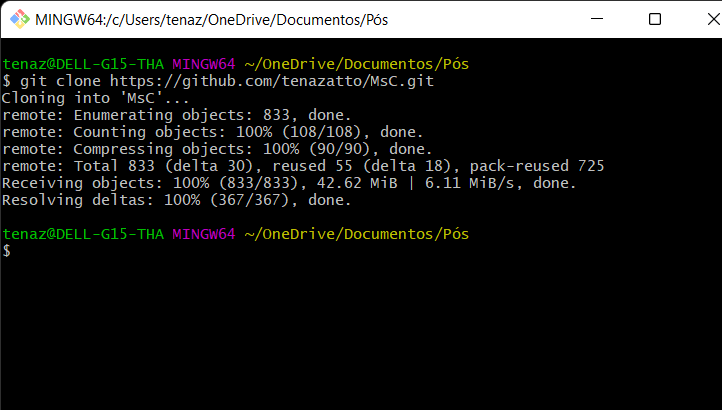
\includegraphics[scale=0.4]{images/git-clone.png}
\label{fig:DocInstallGitClone}
\end{figure}

\subsection{Montagem de ambiente}

Para evitar problemas de versão com bibliotecas de outros projetos instalados, é possível criar um ambiente virtual para realizar a instalação das bibliotecas separadamente. Para criar, é necessário o \textbf{virtualenv} instalado no Python. Caso ele não esteja instalado, ele é obtido através do comando:

\begin{quote}\textbf{pip install virtualenv}\end{quote}

Para criar um novo ambiente virtual, é preciso digitar o comando

\begin{quote}\textbf{python3 -m venv ./(nome do ambiente)}\end{quote}

Como exemplo, nesta documentação foi criado o documento \textbf{testenv}

\begin{figure}[H]
\centering
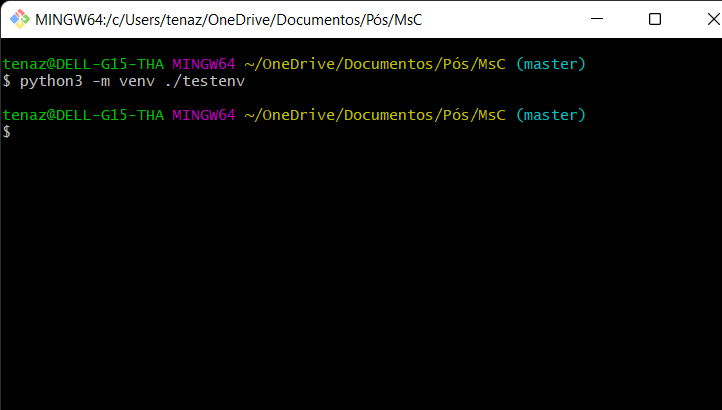
\includegraphics[scale=0.4]{images/virtualenv-sh.png}
\label{fig:DocInstallVirtualEnvShell}
\end{figure}

Após o término, aparecerá uma nova pasta de mesmo nome

\begin{figure}[H]
\centering
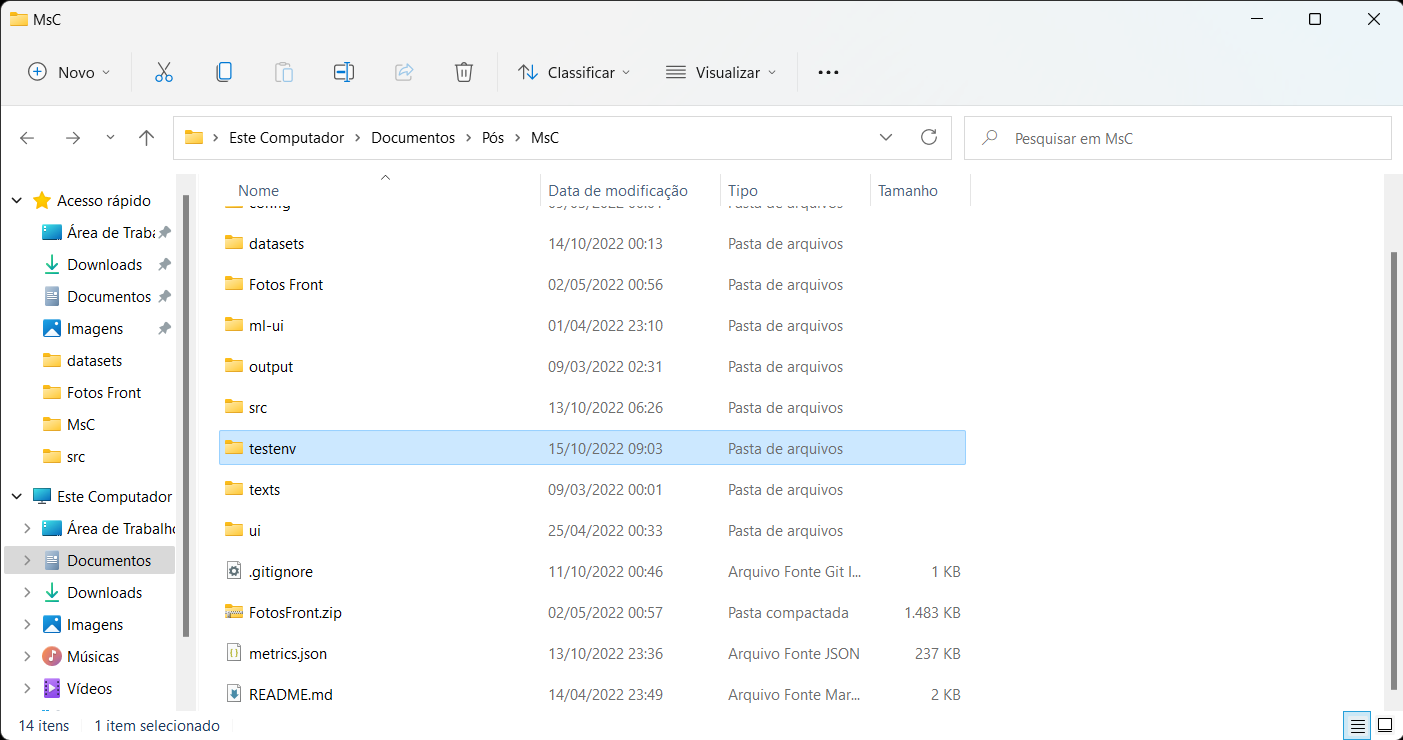
\includegraphics[scale=0.25]{images/virtualenv.png}
\label{fig:DocInstallVirtualEnvFolder}
\end{figure}

Após criar o ambiente virtual, é preciso ativá-lo para utilizar

\begin{quote}
\textbf{.\textbackslash (nome do ambiente)\textbackslash Scripts\textbackslash activate.bat} (Windows - Prompt de Comando)
\end{quote}
\begin{quote}
\textbf{source ./(nome do ambiente)/Scripts/activate} (Windows - Bash)
\end{quote}
\begin{quote}
\textbf{source ./(nome do ambiente)/bin/activate} (Linux)
\end{quote}

Para verificar se o ambiente foi ativado, é possível verificar, ao digitar qualquer comando no bash, que o nome do ambiente virtual aparece logo abaixo.

\begin{figure}[h!]
\centering
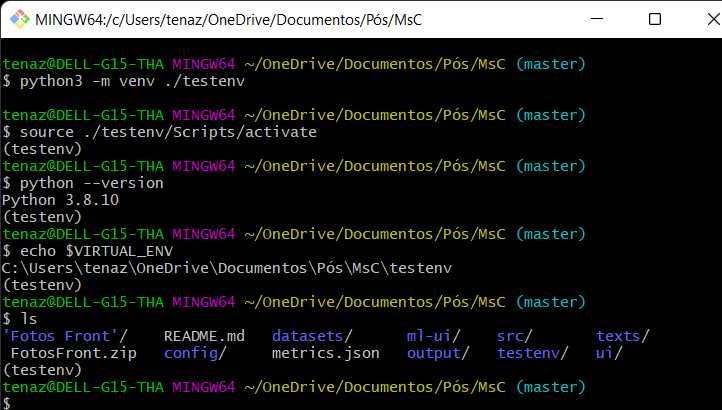
\includegraphics[scale=0.4]{images/virtualenv-check.png}
\label{fig:DocInstallVirtualEnvCheck}
\end{figure}

Para desativar o ambiente virtual, é preciso digitar o comando

\begin{quote}\textbf{deactivate}\end{quote}

Para verificar se o ambiente foi desativado, é possível verificar, ao digitar qualquer comando no bash, que o nome do ambiente virtual não irá mais aparecer até ser ativado novamente.

No caso do Node.js não é necessário realizar tais etapas, pois a instalação das bibliotecas nesta documentação é realizada de maneira local

\subsection{Instalação das bibliotecas}

\subsubsection{Python}

Com o ambiente virtual criado e ativado, é possível utilizar os arquivos \textbf{src/requirements.txt}, dependendo das configurações da sua máquina, para instalar todas as bibliotecas necessárias através do comando

\begin{quote}\textbf{pip install -r ./src/requirements-nvidia.txt} (GPU Nvidia)\end{quote}
\begin{quote}\textbf{pip install -r ./src/requirements-cpu.txt} (CPU)\end{quote}

Estes arquivos foram preparados apenas para rodar de acordo com o hardware apresentado. A execução de ambos os comandos não é necessária e nem recomendável.

\subsubsection{Node.js}

Para o Node.js, como o arquivo \textbf{package.json} está dentro da pasta \textbf{ml-ui}, é possível acessar essa pasta e digitar o comando

\begin{quote}\textbf{npm install}\end{quote}

\section{Execução do sistema}

\subsection{Engenharia de Dados}

Dentro da pasta \textbf{MsC} e com o ambiente virtual criado e ativado, para rodar o módulo de Engenharia de Dados basta digitar o seguinte comando

\begin{quote}\textbf{python -m src.data\_engineering.data\_engineering\_start -{}-data (Opção)}\end{quote}

No momento, há 3 opções disponíveis:

\begin{itemize}
    \item {\textbf{GERMAN\_CREDIT:}} Manipula o German Credit Dataset, cujo arquivo está na localização \textbf{datasets/german.data}, para utilização no Módulo de ML.
    \item {\textbf{LENDINGCLUB:}} Baixa e manipula o Lendingclub Dataset para utilização no Módulo de ML.
    \item {\textbf{METRICS:}} Obtém o maior valor, menor valor e a média de cada métrica para cada execução já realizada no Módulo de ML.
\end{itemize}

\subsection{Módulo de ML}

Dentro da pasta \textbf{MsC}, com o ambiente virtual criado e ativado e com dados já tratados pelo módulo de Engenharia de Dados, para rodar todos os Pipelines presentes no Módulo de ML basta digitar o seguinte comando

\begin{quote}\textbf{python -m src.pipeline.pipeline\_start -{}-dataset (Opção)}\end{quote}

Há 4 opções disponíveis para execução:

\begin{itemize}
    \item {\textbf{ADULT\_INCOME\_SEX:}} Executa os Pipelines do Módulo de ML para o Adult Income Dataset, cujo arquivo está na localização \textbf{datasets/adult.csv}, utilizando Sexo (Masculino/Feminino) como atributo protegido.
    \item {\textbf{GERMAN\_CREDIT\_FOREIGN:}} Executa os Pipelines do Módulo de ML para o German Credit Dataset, cujo arquivo é manipulado na etapa anterior, utilizando Nacionalidade (Alemão/Estrangeiro) como atributo protegido.
    \item {\textbf{GERMAN\_CREDIT\_AGE:}} Executa os Pipelines do Módulo de ML para o German Credit Dataset, cujo arquivo é manipulado na etapa anterior, utilizando Idade (-25 anos/25 ou + anos) como atributo protegido.
    \item {\textbf{LENDINGCLUB\_INCOME:}} Executa os Pipelines do Módulo de ML para o Lendingclub Dataset, cujo arquivo é manipulado na etapa anterior, utilizando Renda (-1 salário mínimo/1 ou + salários mínimos) como atributo protegido.
\end{itemize}

Após a execução, é possível ver a geração das métricas dentro da pasta \textbf{output/metrics}, necessárias para a execução do Gerenciador Autonômico.

\begin{figure}[H]
\centering
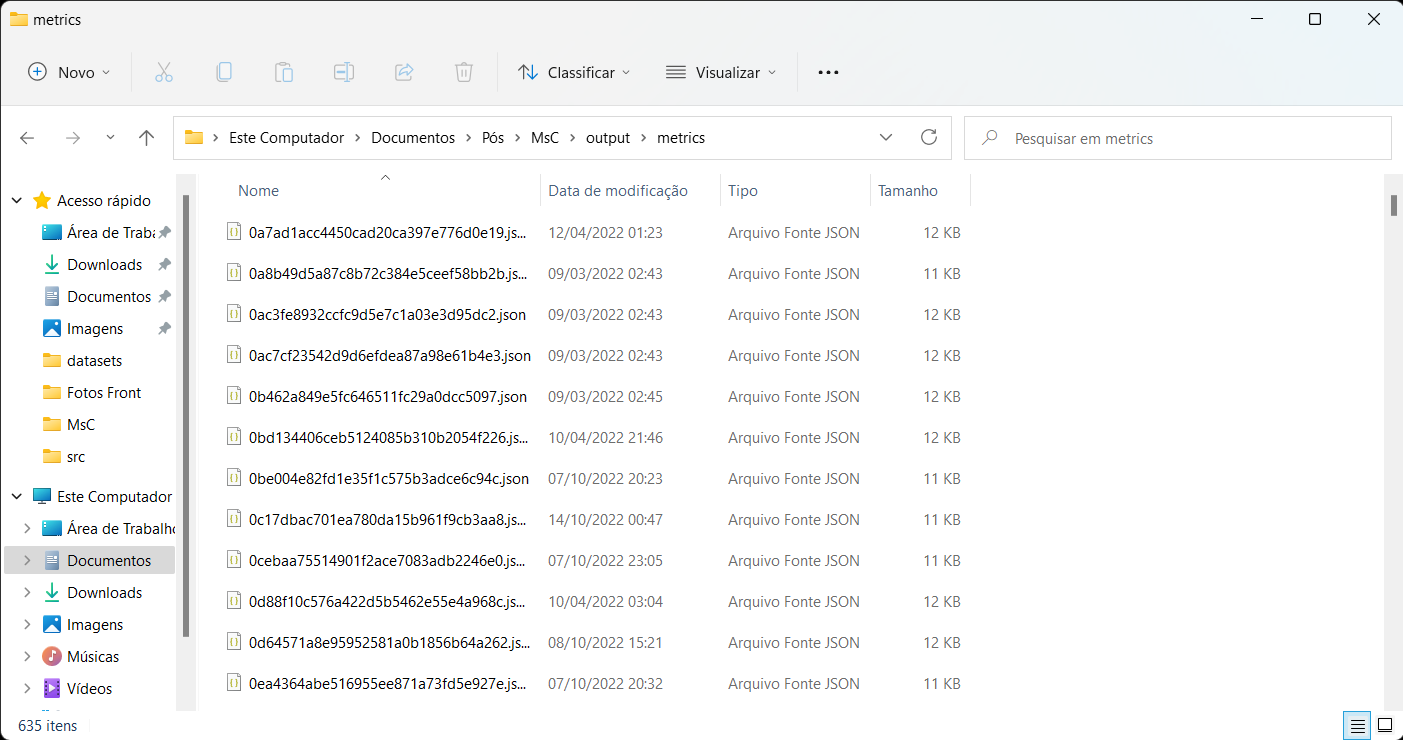
\includegraphics[scale=0.25]{images/metrics.png}
\label{fig:DocInstallMetrics}
\end{figure}

\subsection{Gerenciador Autonômico}

Dentro da pasta \textbf{MsC}, com o ambiente virtual criado e ativado e com pelo menos uma execução do Módulo de ML realizada, é possível verificar como o Gerenciador Autonômico funciona com o seguinte comando

\begin{quote}\textbf{python -m src.mapek.mapek\_start}\end{quote}

Nesta etapa, ele escolhe o Pipeline que apresentou as melhores métricas, porém a filtragem por conjunto de dados foi desenvolvida apenas na Interface. Como ele roda ininterruptamente, é preciso interromper sua execução.

\subsection{Interface}

\subsubsection{Backend}

Dentro da pasta \textbf{MsC}, com o ambiente virtual criado e ativado e com pelo menos uma execução do Módulo de ML realizada, é possível rodar o Backend da interface com o seguinte comando

\begin{quote}\textbf{python -m src.api.flask\_start}\end{quote}

Ele vai iniciar um servidor na porta 8080, necessário para rodar as requisições que o Frontend vai solicitar

\begin{figure}[H]
\centering
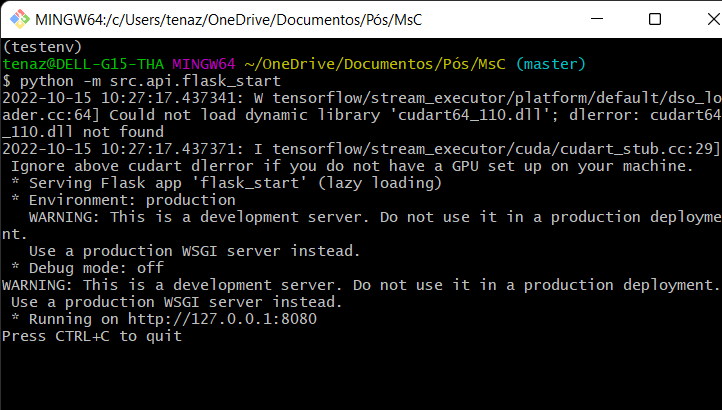
\includegraphics[scale=0.4]{images/backend-start.png}
\label{fig:DocInstallVirtualEnvBackendStart}
\end{figure}

\subsubsection{Frontend}

Dentro da pasta \textbf{MsC/ml-ui}, é possível rodar o Frontend da interface com o seguinte comando

\begin{quote}\textbf{npm start}\end{quote}

Ele vai iniciar o navegador acessando um servidor na porta 3000, e deverá iniciar a tela no menu de Análise

\begin{figure}[H]
\centering
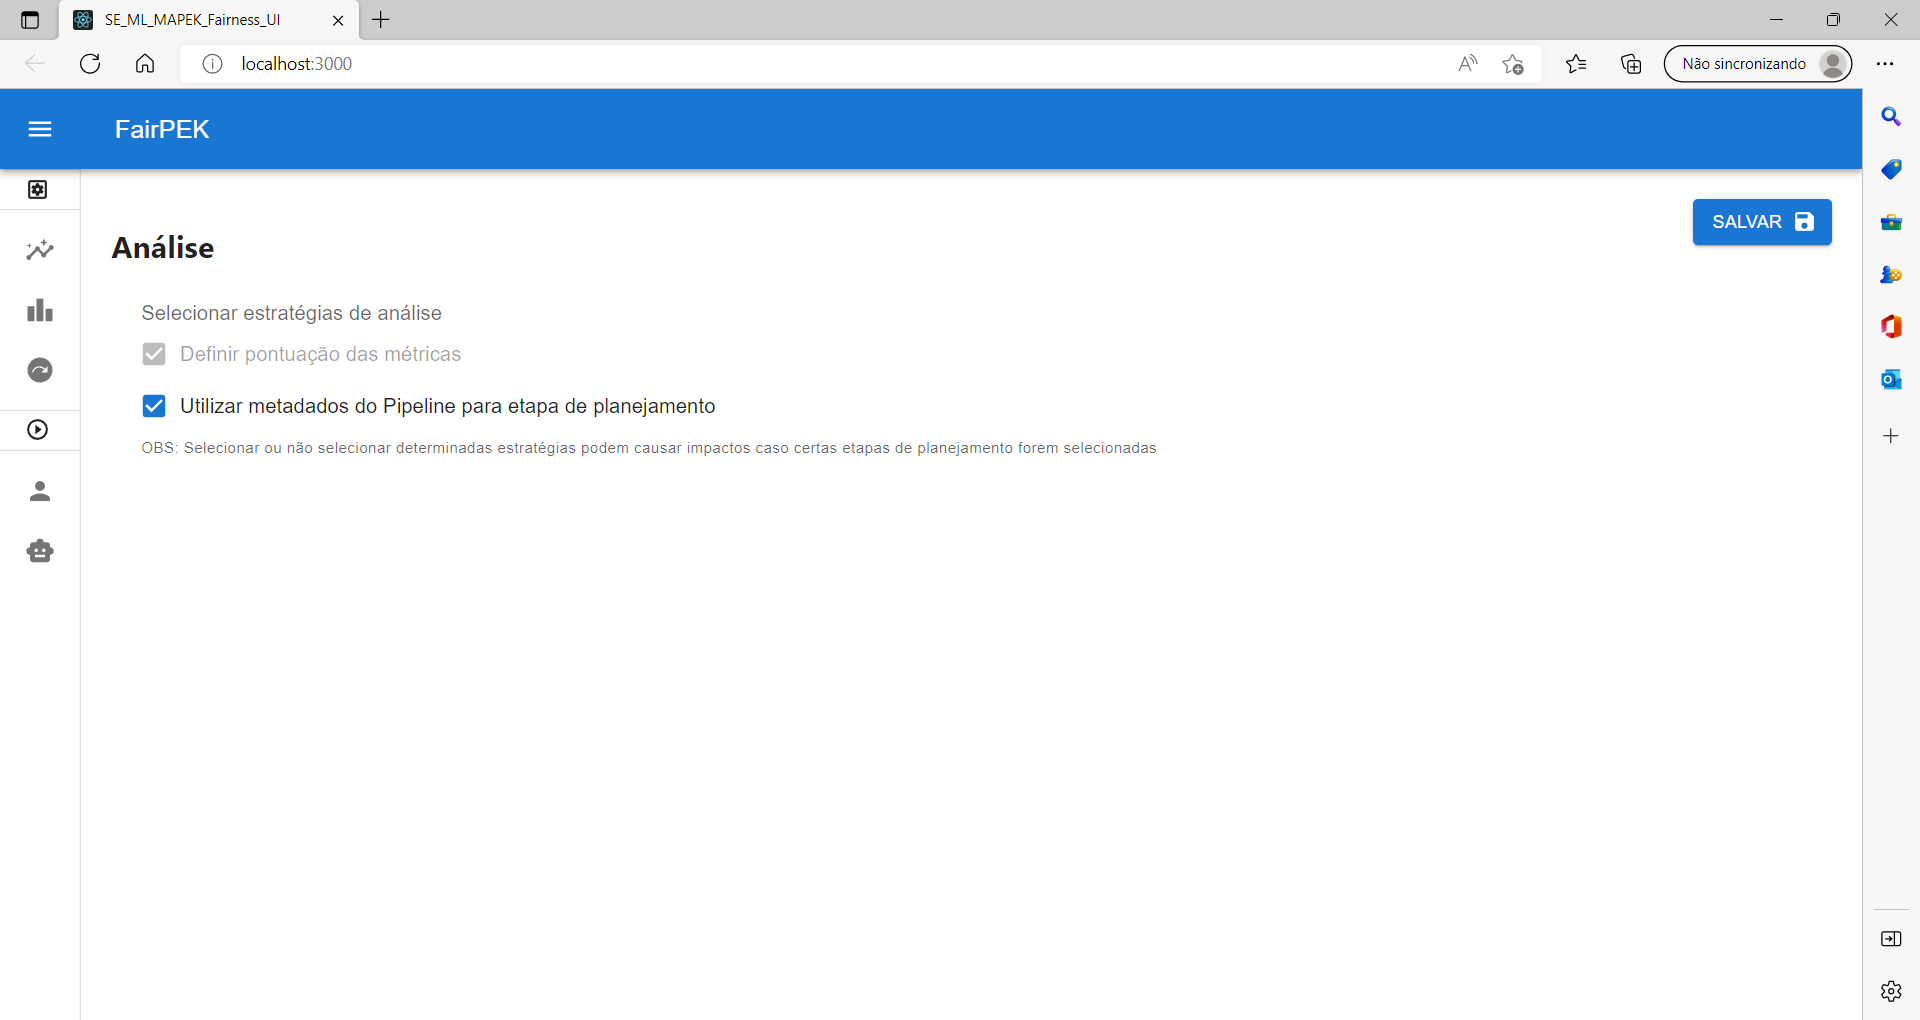
\includegraphics[scale=0.3]{images/ml-ui.png}
\label{fig:DocInstallMLUI}
\end{figure}

\end{document}


